\documentclass[designspec/spec.tex]{subfiles}

%Sammanfattningen bör innehålla:
%
%   -En beskrivning av de mest framträdande egenskaperna hos det totala
%   systemet och de olika delsystemen.
%
%   -Ett blockschema som beskriver konstruktionens uppdelning i olika delar.
%
%   -En beskrivning av vilka sensorer som ska användas och hur de ska placeras.
%
%   -En beskrivning av vilka ställdon (motorer etc,) som ska användas och hur
%   de ska användas och hur de ska placeras.

\begin{document}

\section{Översikt}
I denna del förklaras designen av systemet översiktligt.

\subsection{Framträdande egenskaper}
Produkten består av tre moduler: Kommunikation-, sensor- och styrmodul.
Sensormodulen kommer implenteras på ett virkort varav de andra modulerna ska
vara på ett separat virkort. Produkten har två avståndsmätare och en kamera
till hjälp när produkten ska samla in information om sin omgivning. Vardera
mikrokontroller klockas med en kristalloscillator. Produkten är ansluten till en
fjärrklient via WLAN.

\begin{figure}[h]
    \centering
    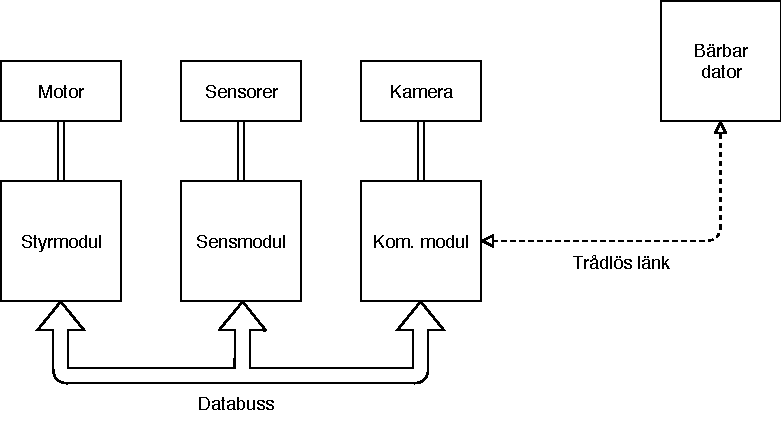
\includegraphics[width=0.6\linewidth]{designspec/fig/blockskiss.pdf}
    \caption{Övergripande bild över systemet och dess moduler. SPI-buss används}
    \label{fig:overview}
\end{figure}
\noindent
Kommunikationsmodulen består av en Raspberry Pi och kommer vara en central
kommun\-ikations- och beslutsenhet som ansvarar för att ta beslut om taxins
beteende samt hantera kommunikationen mellan modulerna. Styrmodulen består av
motorer och en mikrokontroller och står för drift samt reglering av taxins
hastighet och svängradie. Sensormodulen består av en mikrokontroller samt
avståndsmätare och halleffektsensorer monterade på bilens hjul.

\subsection{Sensorer}
Kameran ska fästas en bit ovan alla korten och titta framåt med en vinkel
nedåt. Avståndsmätaren som ska mäta avstånd till hinder ska fästas på framsidan
av bilens chassi. Om det behövs så ska lämpliga fotfästen skrivas ut med en
3D-skrivare. Den andra avståndsmätaren ska användas för att avgöra när ett
hinder har passerats vid omkörning och kommer att placeras på bakre höger sida
av bilens chassi. Odometern som används till att mäta kördistans är redan
färdigmonterad på chassit.

\subsection{Ställdon}
Hjulen, motorerna och ställdonen är redan färdigmonterade. Motorerna används
för att få bilen att åka framåt och bakåt samt för att svänga.

\end{document}
